\documentclass[12pt,a4paper]{article}
\usepackage{graphicx}
\usepackage{amsmath, amssymb}
\usepackage{siunitx}
\usepackage{geometry}
\geometry{margin=2.5cm}
\usepackage{wrapfig}
\usepackage{caption}
\usepackage{subcaption}

\captionsetup[figure]{width=0.8\textwidth}  % for all figures

\begin{document}
\title{Plumbus creation through the use of 3D scanning, FDM printing and
laser-cutting}

\author{
  BSc-5 \\[1em]
  Adam Gabor Bacso \\
  Borys Maksymilian Bobrowski \\
  Greta Klara Wodala \\
  Juan Ruiz \\
  Nikola Dragomirov Dimitrov \\
  Rui Emanuel Vasquez Pacheco
}

\date{October, 2025}
\maketitle
\tableofcontents
\newpage

\section{Introduction}

The goal of the project was to create a 3D printed plumbus -- a fictional
household item from the Rick and Morty universe -- by 3D scanning at least 5
common, physical objects. The scanned files needed to be fabricated using a
Fused Deposition Modeling (FDM) printer along with a base for the object by the
method of laser-cutting.

A plumbus has 5 distinct parts for which 5 real world items have been selected:

\begin{figure}[h]
  \begin{center}
    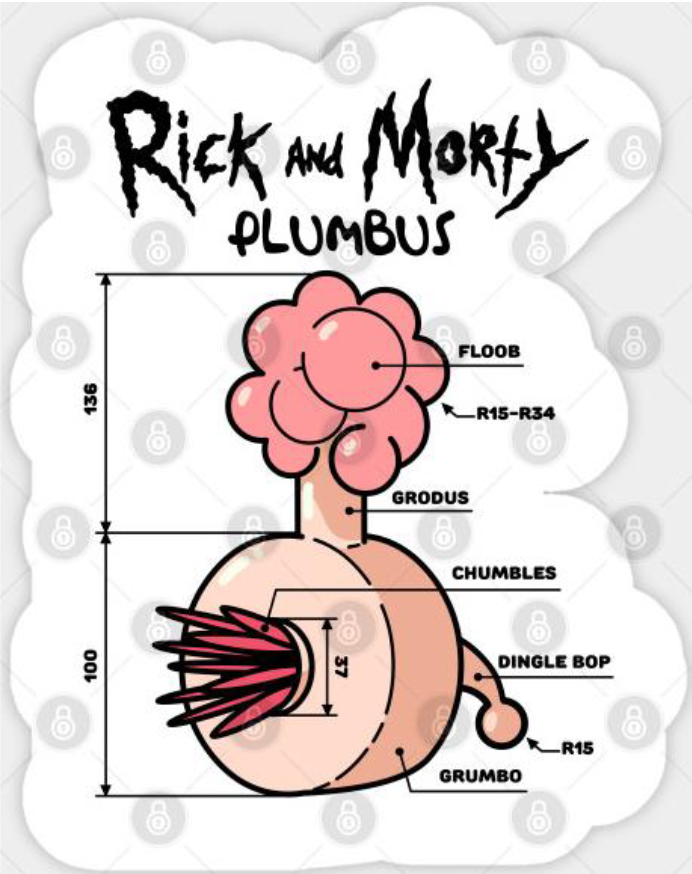
\includegraphics[width=0.4\linewidth]{media/plumbus_drawing.png}
  \end{center}
  \caption{Labeled image of a plumbus with rough dimensions.}
\end{figure}

\begin{itemize}
  \item Floob $\to$ microfiber cloth ball
  \item Grodus $\to$ toiletpaper roll core
  \item Chumbles $\to$ brush bristles
  \item Dingle bop $\to$ microfiber cloth cone
  \item Grumbo $\to$ toiletpaper roll
\end{itemize}

Objects were chosen from common cleaning supplies to reflect some of the uses of
the plumbus.

\section{Scanning}

The first step in creating the plumbus was to acquire the geometries of the
selected objects.

First, the objects had to be prepared to fit the exact needs of the project. For
some, such as the paper tube, it meant creating additional, more detail-rich
texture while for others it meant modifying their shape and adding a mounting
option to allow scanning on all sides. Most of these modifications were made
with the use of rubber bands.

The first method of 3D scanning was to attempt photogrammetry
with mobile devices. The main issue encountered was the impossibly long upload a
processing times of the apps\footnote{Apps attempted were Polycam, Modelar and
CamToPlan.} that we tried. Blaming the server-based processing, the use of
\emph{Meshroom} was attempted for stitching individual images into a 3D scene,
but it also abandoned due to its extreme hardware and storage requirements.

Finally, a decision has been made to use specialized scanning hardware.
The scanner used was the \emph{EINSTAR VEGA hand scanner},
provided by our professor. With its display and on-device processing, it proved
to be fairly user-friendly, but several issues also presented themselves.

\begin{figure}[h]
  \centering
  \includegraphics[width=0.3\textwidth]{media/scanning.png}
  \caption{The UI of the EINSTAR VEGA gave valuable information such as the
    optimal distance to the scanned object as well as areas that still need more
  definition.}
\end{figure}

\renewcommand{\arraystretch}{2}
\begin{table}[h]

  \centering
  \begin{tabular}{ | p{0.35\linewidth} | p{0.6\linewidth} | }
    \hline
    Issue & Solution \\
    \hline
    Scans would not initiate/not recognize an object's presence. & Starting
    scans from the pedestal used (chair) and only after initialization moving up
    to the desired object. \\
    When scanning the hanging ball, the chair leg obstructed the view to the
    object. & Switching to a detailed scan reduced the working distance.\\
    Some objects, mainly those of paper, lost tracking easily. & Adding dots on
    the exteriors seemed to facilitate tracking by adding distinct features for
    texture based tracking.\\
    \hline
  \end{tabular}
  \caption{List of issues faced with the actions taken to tackle the problem.}
\end{table}

\end{document}
